\usetikzlibrary{angles,quotes,decorations.pathreplacing}
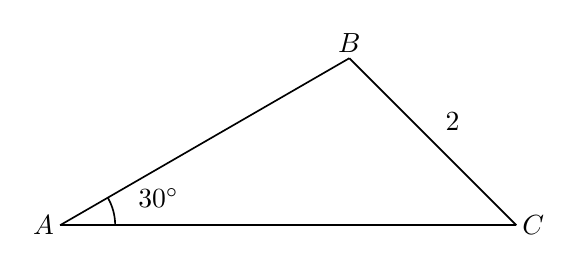
\begin{tikzpicture}[x=1cm,y=1cm,font=\normalsize,
 geometry edge/.style={solid,line width=.6pt},
 geometry mark/.style={solid,line width=.6pt},
 geometry label/.style={font=\normalsize,inner sep=2pt}]
\coordinate (A) at (0.0,0.0);
\coordinate (B) at (3.674234614,2.121320344);
\coordinate (C) at (5.795554958,0.000000000);
\coordinate (LA) at (1.250000000,0.340000000);
\coordinate (L2) at (4.984894786,1.310660172);
\draw[geometry edge] (A)--(B);
\draw[geometry edge] (B)--(C);
\draw[geometry edge] (C)--(A);
\pic[draw, geometry mark, angle radius=7mm] {angle=C--A--B};
\node[geometry label,left] at (A) {$A$};
\node[geometry label,above] at (B) {$B$};
\node[geometry label,right] at (C) {$C$};
\node[geometry label] at (LA) {$30^\circ$};
\node[geometry label] at (L2) {$2$};
\end{tikzpicture}
